 \setlength{\baselineskip}{20pt}
\chapter{常用的命令样例}
\label{cha:chap2}

论文撰写规范参照《北京交通大学学位论文撰写规范》,以下简称《规范》。下面整理了论文撰写过程中常用的一些命令样例,以便论文撰写者查阅使用。
《北京交通大学学位论文撰写规范》见https://gs.bjtu.edu.cn/cms/item/477.html

\section{中文\cp{全角}括弧}
为了避免正文中直接写中文括弧出现的文字光标错位问题,本模板制定了两种中文括弧的命令,建议在正文中使用命令来实现中文括弧:

\textbf{半括弧},\textbackslash rp\{1\}:\rp{1}xxx。\rp{2}xxx。

\textbf{全括弧},\textbackslash cp\{1\}:\cp{1}xxx。\cp{2}xxx。

\section{公式}

公式规范参照《规范》中3.10.12节。本模板定义了一些常用的命令,包括向量、矩阵、张量、引用公式命令。下面展示一些样例,便于论文撰写者使用:

\textbf{向量},\textbackslash vec\{x\}:$\vec{x}$

\textbf{矩阵},\textbackslash mat\{x\}:$\mat{X}$

\textbf{张量},\textbackslash tensor\{x\}:$\tensor{X}$

\textbf{引用公式},引用公式时需要带有全角括号,可使用本模板定义的\textbackslash refeq命令,自带全角括号,例子:如公式\refeq{eq:ch2-split}所示。

\textbf{较长的上下标},应使用非斜体\textbackslash mathrm\{xxx\},如:$\vec{x}_{\mathrm{example}}^{\mathrm{example}}$。


%\begin{equation}\label{eq:ch2-example}
%	\vec{x}_{\mathrm{example}}^{\mathrm{example}}
%\end{equation}

\textbf{嵌入在文本中的公式},使用\$\$命令,例子:$a + b = c$。

\textbf{单独为行的公式},使用\textbackslash begin\{equation\}和\textbackslash end\{equation\}命令,较长的公式需要转行时,应尽可能在“$ = $”处回行,或者在“$ + $”、“$-$”“$*$”等记号处回行。例子:如公式\refeq{eq:ch2-split}、公式\refeq{eq:ch2-aligned}和公式\refeq{eq:ch2-align}所示。

\begin{equation}\label{eq:ch2-aligned}
	\begin{aligned}
		\dot{\hat{A}}^\dag
		&=\lambda_1\left(\tanh(k_3e_v)e_v-\sigma_1\hat{A}^\dag\right)\\
		&=\lambda_1\tanh(k_3e_v)e_v-\lambda_1\sigma_1\hat{A}^\dag
	\end{aligned}
\end{equation}

\begin{equation}\label{eq:ch2-split}
	\left\{
	\begin{split}
		\frac{\texttt{d}p(t)}{\texttt{d}t}&=v(t)\\
		\frac{\texttt{d}v(t)}{\texttt{d}t}&=u(t)-a(t)-b(t)v(t)-c(t)v^2(t)-f_2^*(\cdot)
	\end{split}
	\right.
\end{equation}




\begin{subequations}\label{eq:ch2-align}
	\begin{align}
		\dot{\hat{A}}^\dag&=\lambda_1\left(\tanh(k_3e_v)e_v-\sigma_1\hat{A}^\dag\right)\\
		\dot{\hat{b}}^\dag&=\lambda_2\left(|v||e_v|-\sigma_2\hat{b}^\dag\right)\\
		\dot{\hat{c}}^\dag&=\lambda_3\left(v^2|e_v|-\sigma_3\hat{c}^\dag\right)
	\end{align}
\end{subequations}

%
%\section{图片}
%
%图片规范参照《规范》中3.10.4节,图题采用中英文对照,中文在上,居中书写,英文\cp{Times New Roman}字体五号,中文宋体五号。
%
%图中文字用宋体(中文)或Times New Roman字体(英文),字号尽量采用5号字(当字数较多时可用小5号字,以清晰表达为原则,但在一个插图内字号要统一)。同一图内使用文字应统一。图表中物理量、符号用斜体。
%
%插图之前,文中必须有关于本插图的提示,如“见图1-1”、“如图1-1所示”等。插图与其图题为一个整体,不得拆开排写于两页。插图处的该页空白不够排写该图整体时,则可将其后文字部分提前排写,将图移到次页。有分图时,分图过多在一页内安排不下时,可转到下页,总图题只出现在下页。
%
%\textbf{单图},如图\ref{fig:ch2-f1}所示。
%
%\textbf{多图并列},如图\ref{fig:ch2-f2}所示。
%
%\textbf{巨型图},为了美观,超大规模的图可尝试旋转独占一页,本模板已添加旋转包,只需将\textbackslash begin\{figure\}和\textbackslash end\{figure\}命令中的figure换为sidewaysfigure即可。
%
%\begin{figure}[!htb]
%	\centering
%	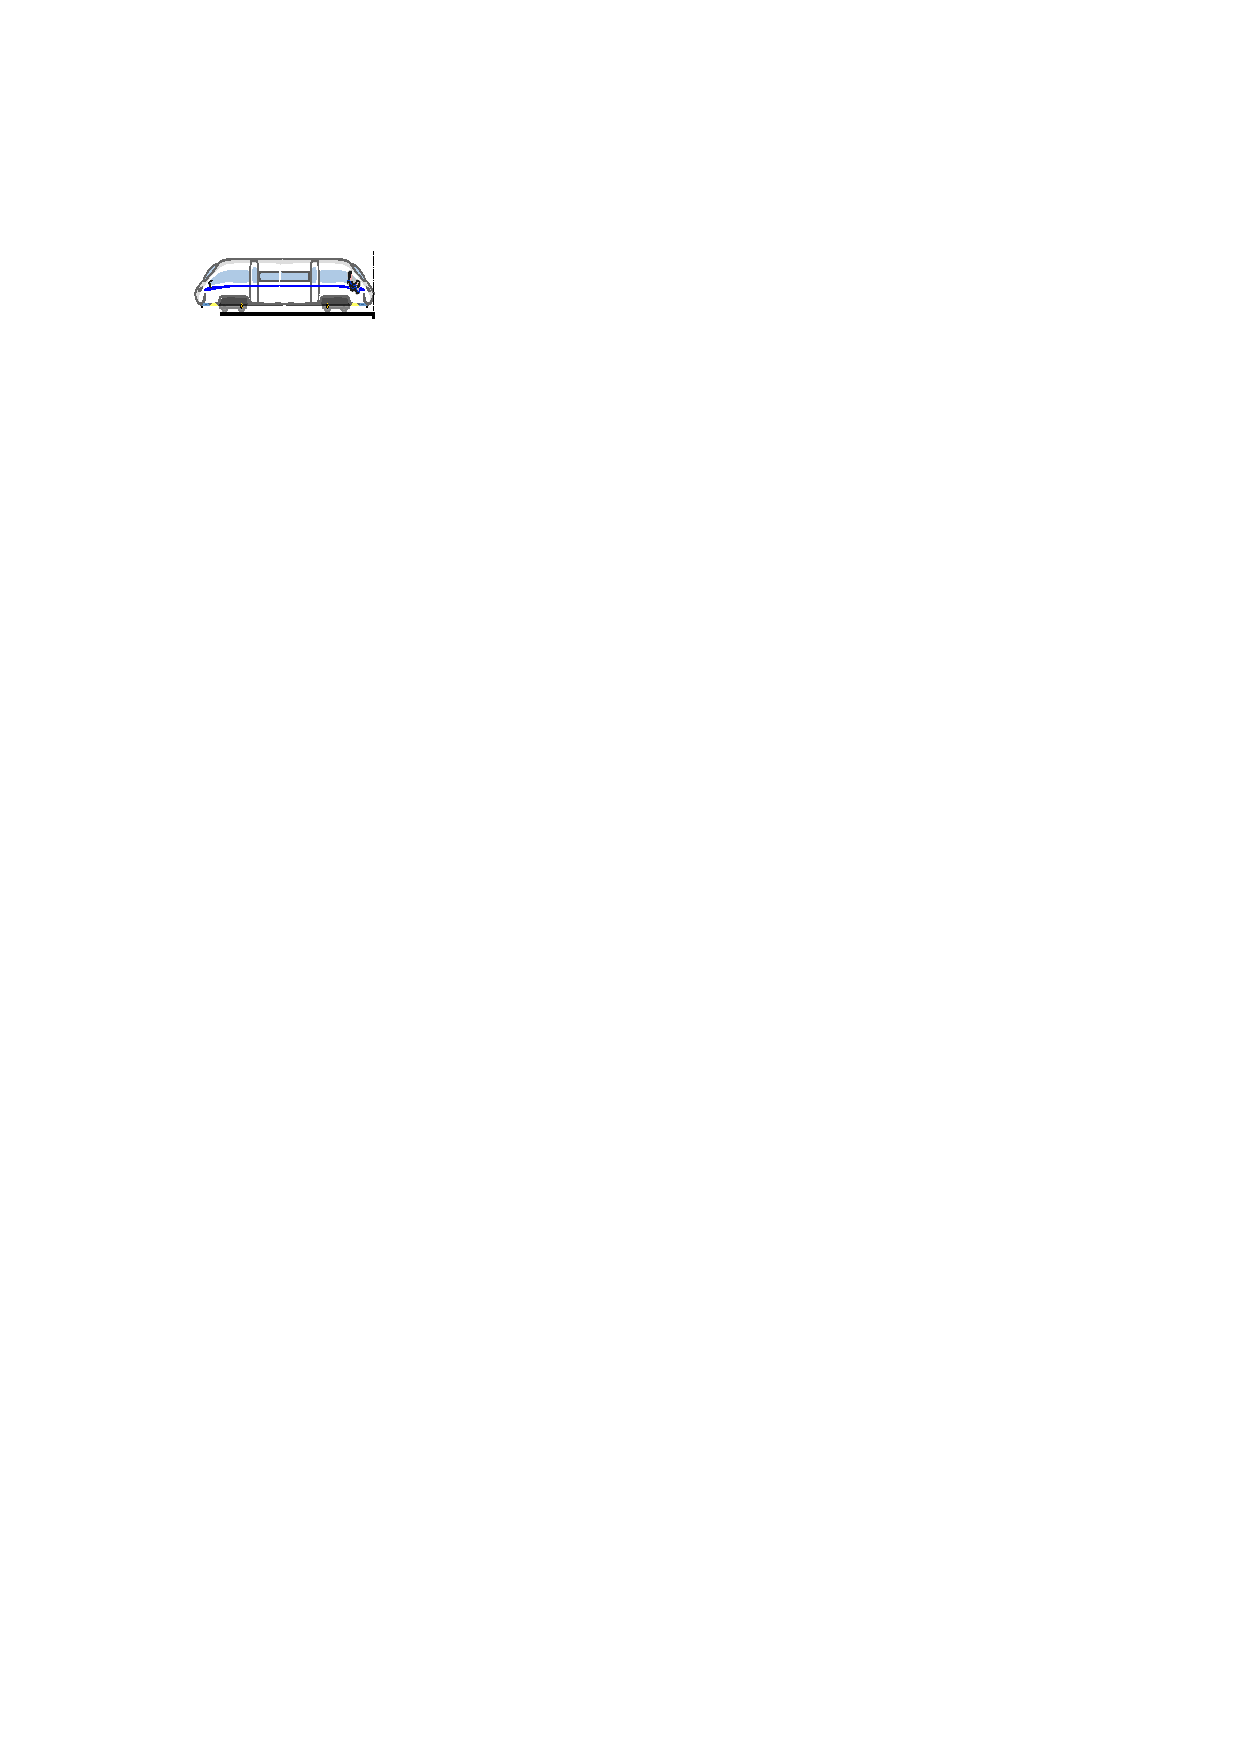
\includegraphics[scale=0.95]{figures/ch2/figure1.pdf}
%	\caption{xxx示意图。 \\Fig~\ref{fig:ch2-f1}~Illustration of xxx.}
%	\label{fig:ch2-f1}
%\end{figure}
%
%\begin{figure}[!htb]
%	\centering
%	\setlength{\belowcaptionskip}{-0.2cm} %调整图片caption与正文之间的间距,table用\abovecaptionskip。可自己调整。
%	\addtocounter{subfigure}{-1}\subfigure[Subfig1.] {\subfigure[子图1] {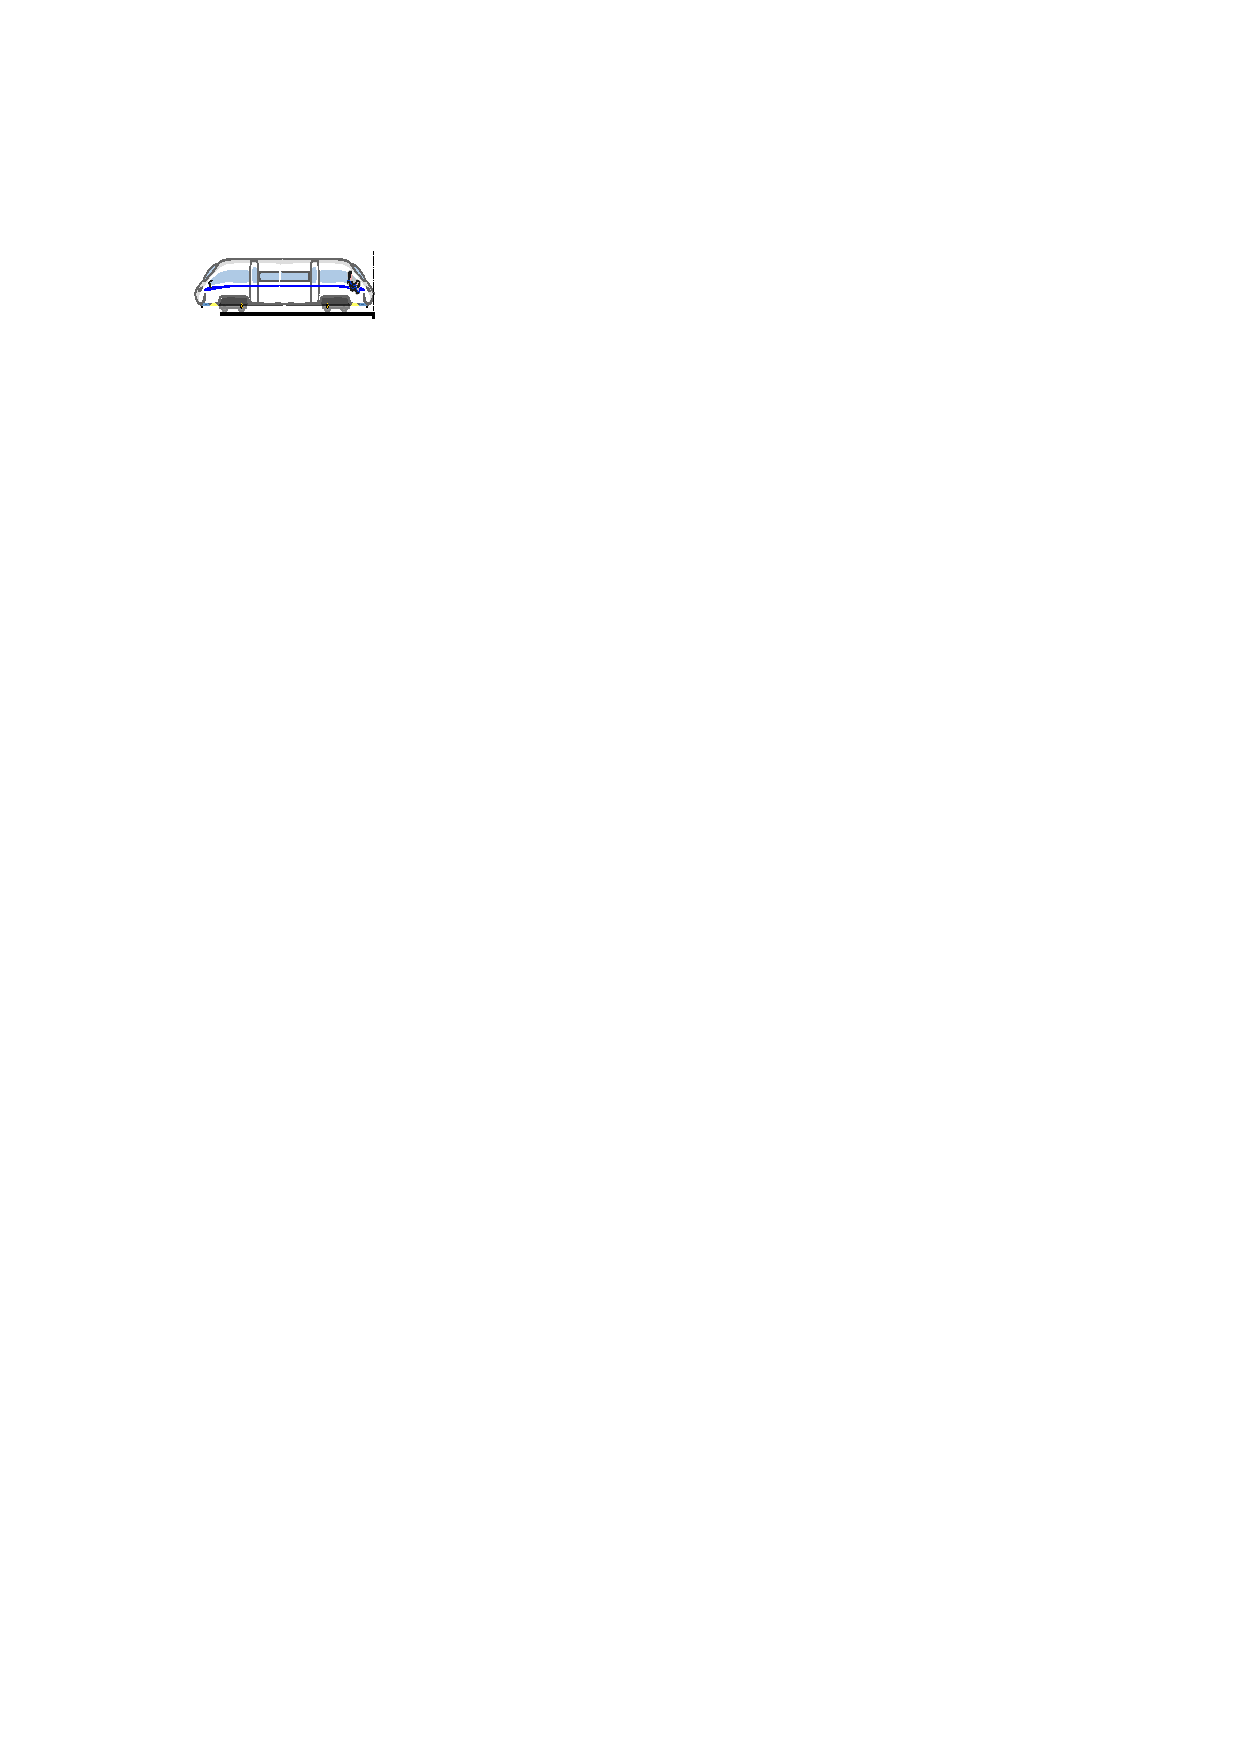
\includegraphics[scale=1]{figures/ch2/figure1.pdf}}}
%	\hspace{20pt} %子图间距
%	\addtocounter{subfigure}{-1}\subfigure[Subfig2.] {\subfigure[子图2]{ 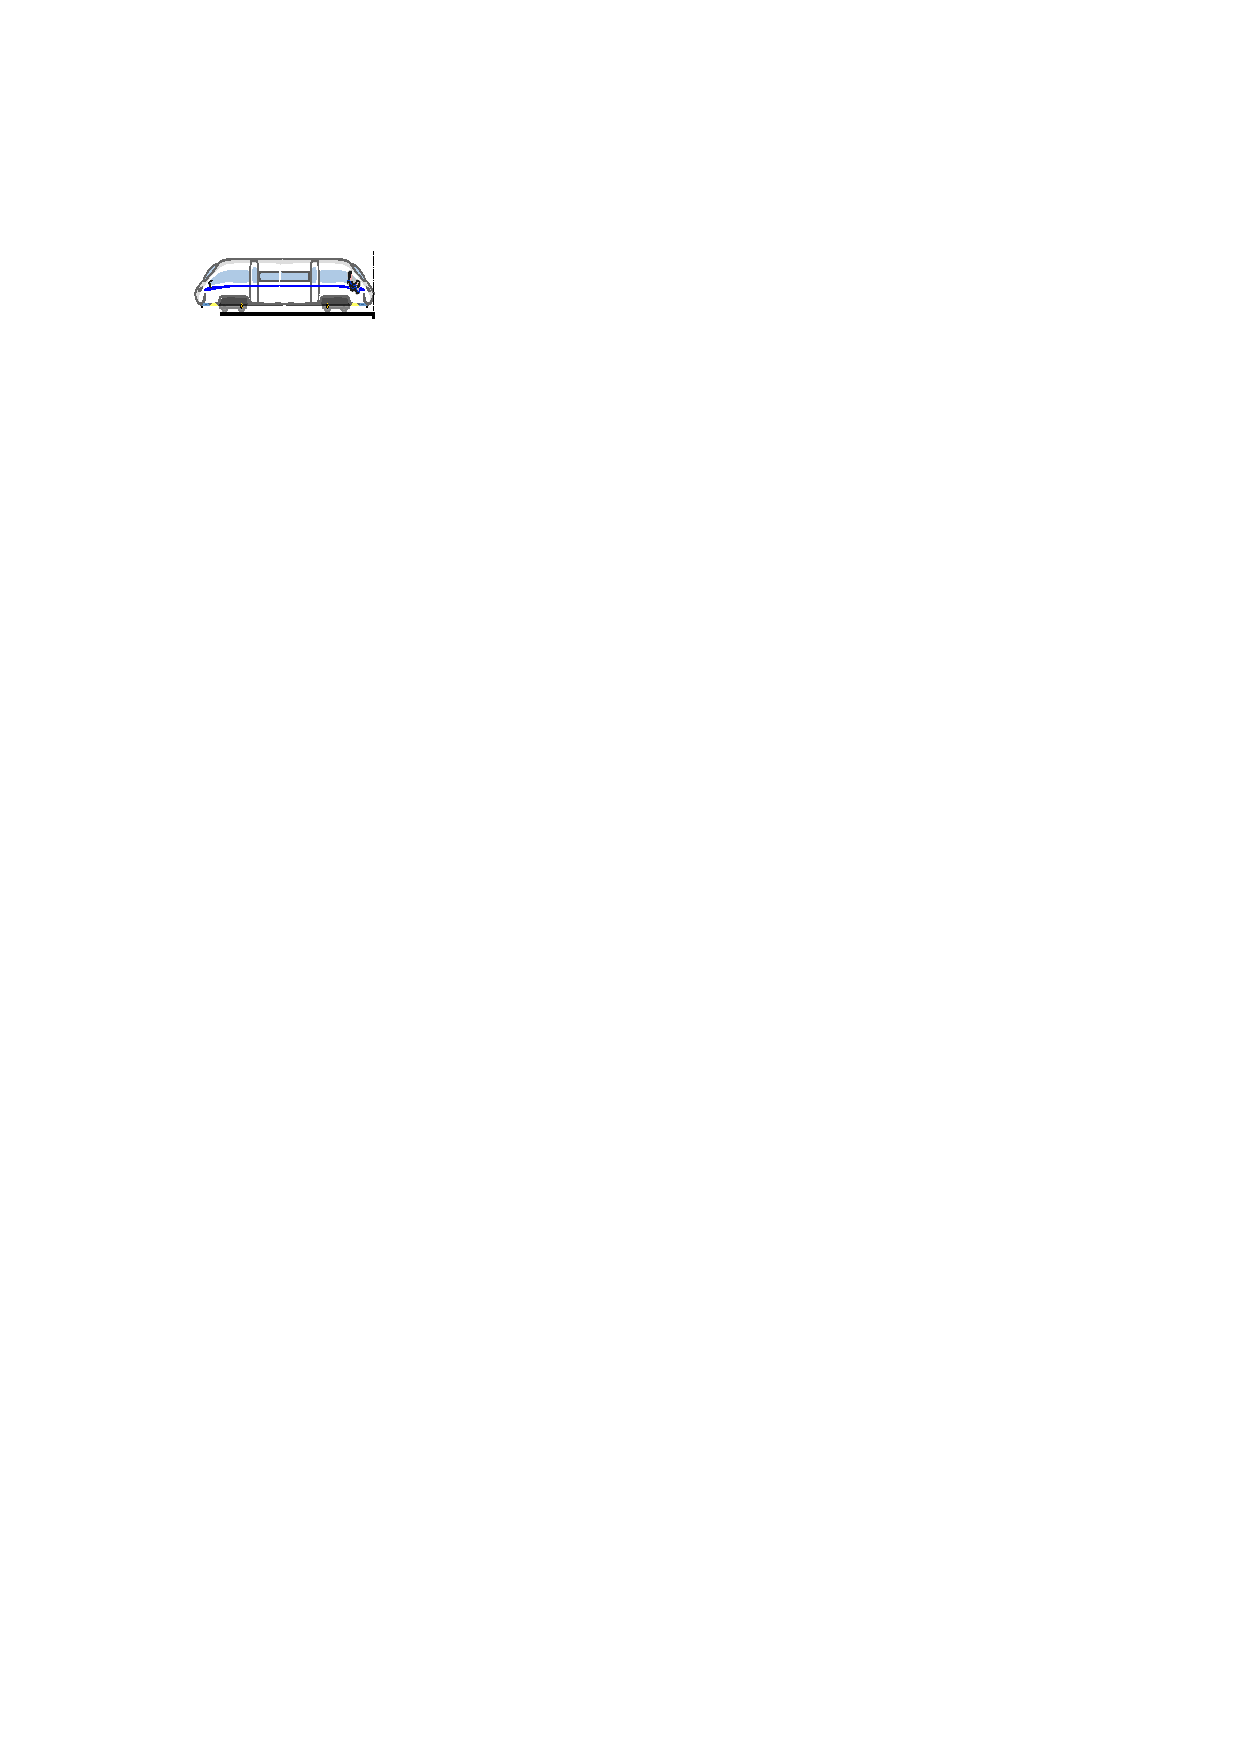
\includegraphics[scale=1]{figures/ch2/figure1.pdf}}}
%	\caption{xxx示意图。\\Fig~\ref{fig:ch2-f2}~Illustration of xxx.}
%	\label{fig:ch2-f2}
%\end{figure} 

\section{定理}


\begin{Definition}
	这是一个定义。
\end{Definition}

\begin{Theorem}
	这是一个引理。
\end{Theorem}

\begin{Proof}
	这是一个证明。
	\qed
\end{Proof}

\section{表格}

表格规范参照《规范》中3.10.5节。表题采用中英文对照,置于表的上方,居中,中文在上。英文(Times New Roman)字体五号,中文宋体五号。 

表格的编排建议采用国际通行的三线表,不加左、右边框线。表中文字用宋体(中文)或Times New Roman字体(英文),字号尽量采用5号字(当字数较多时可用小5号字,同一个插表内字号要统一)。

\textbf{普通的三线表}:如表\ref{tab:ch2_res1}所示。如果表格超出页面边距或内容太过拥挤,可以使用\textbackslash tabcolsep命令来调节列间距。

\textbf{带脚注的三线表}:如表\ref{tab:ch2_res2}所示,标题中写不下的内容可放至脚注,此时使用threeparttable包来实现。

\textbf{巨型表格}:表格过大且无法拆分成多个表格时,可以使用sidewaystable旋转表格独占一页,本模板已添加旋转包,只需将\textbackslash begin\{table\}和\textbackslash end\{table\}命令中的table换为sidewaystable即可。如表\ref{tab:ch2_res3}所示。

%\begin{table}[!htb]
%	\small %字体大小
%	%\setlength\tabcolsep{3.3pt} %调整列间距
%	\caption{性能对比。\\Table~\ref{tab:ch2_res1}~Performance comparison. }
%	\begin{tabular}{c|ccc|ccc}
%		\toprule
%		\multirow{2}{*}{模型} &  & 数据集1 &  &  & 数据集2&  \\
%		& MAE & RMSE & MAPE(\%) & MAE & RMSE & MAPE(\%) \\
%		\midrule
%		
%		SVR & 46.46 & 92.97 & 83.40 & 11.10 & 19.84 & 91.96  \\
%		LSTM & 36.20 $\pm$0.17 & 66.26 $\pm$0.80 & 40.42 $\pm$0.86 & 6.70 $\pm$0.02 & 11.36 $\pm$0.04 & 74.01 $\pm$1.26  \\
%		\bottomrule
%	\end{tabular}
%	\label{tab:ch2_res1}
%\end{table}

\begin{table}[!htb]
	\centering
	\small %字体大小
	\setlength\tabcolsep{10pt} %调整列间距
	\caption{性能对比。\\Table~\ref{tab:ch2_res1}~Performance comparison. }
	\begin{tabular}{c|ccc}
		\toprule
		模型 & MAE & RMSE & MAPE(\%)  \\
		\midrule
		LSTM & 36.20 $\pm$0.17 & 66.26 $\pm$0.80 & 40.42 $\pm$0.86 \\
		\bottomrule
	\end{tabular}
	\label{tab:ch2_res1}
\end{table}

\begin{table}[!htb]
	\centering
	\small %字体大小
	%\setlength\tabcolsep{3.3pt} %调整列间距
	\caption{性能对比。\\Table~\ref{tab:ch2_res2}~Performance comparison. }
	\begin{threeparttable}
		\begin{tabular}{c|ccc|ccc}
			\toprule
			\multirow{2}{*}{模型} &  & 数据集1 &  &  & 数据集2&  \\
			& MAE & RMSE & MAPE(\%) & MAE & RMSE & MAPE(\%) \\
			\midrule
			
			SVR & 46.46 & 92.97 & 83.40 & 11.10 & 19.84 & 91.96  \\
			LSTM & \textbf{36.20 $\pm$0.17} & \textbf{66.26 $\pm$0.80} & \textbf{40.42 $\pm$0.86} & \textbf{6.70 $\pm$0.02} & \textbf{11.36 $\pm$0.04} & \textbf{74.01 $\pm$1.26}  \\
			\bottomrule
		\end{tabular}
		\begin{tablenotes}
			\footnotesize
			\item[*] 粗体代表所有基准模型中的最佳的性能。
		\end{tablenotes}
	\end{threeparttable}
	\label{tab:ch2_res2}
\end{table}



% 独占一页的表格样例
\begin{sidewaystable}[!htp]
	%\small %字体大小
	\setlength\tabcolsep{20pt} %调整列间距
	\caption{性能对比。\\Table~\ref{tab:ch2_res3}~Performance comparison. }
	\begin{threeparttable}
		\begin{tabular}{c|ccc|ccc}
			\toprule
			\multirow{2}{*}{模型} &  & 数据集1 &  &  & 数据集2&  \\
			& MAE & RMSE & MAPE(\%) & MAE & RMSE & MAPE(\%) \\
			\midrule
			
			SVR & 46.46 & 92.97 & 83.40 & 11.10 & 19.84 & 91.96  \\
			LSTM & 36.20 $\pm$0.17 & 66.26 $\pm$0.80 & 40.42 $\pm$0.86 & 6.70 $\pm$0.02 & 11.36 $\pm$0.04 & 74.01 $\pm$1.26  \\
			LSTM & 36.20 $\pm$0.17 & 66.26 $\pm$0.80 & 40.42 $\pm$0.86 & 6.70 $\pm$0.02 & 11.36 $\pm$0.04 & 74.01 $\pm$1.26  \\
			LSTM & 36.20 $\pm$0.17 & 66.26 $\pm$0.80 & 40.42 $\pm$0.86 & 6.70 $\pm$0.02 & 11.36 $\pm$0.04 & 74.01 $\pm$1.26  \\
			LSTM & 36.20 $\pm$0.17 & 66.26 $\pm$0.80 & 40.42 $\pm$0.86 & 6.70 $\pm$0.02 & 11.36 $\pm$0.04 & 74.01 $\pm$1.26  \\
			LSTM & 36.20 $\pm$0.17 & 66.26 $\pm$0.80 & 40.42 $\pm$0.86 & 6.70 $\pm$0.02 & 11.36 $\pm$0.04 & 74.01 $\pm$1.26  \\
			LSTM & 36.20 $\pm$0.17 & 66.26 $\pm$0.80 & 40.42 $\pm$0.86 & 6.70 $\pm$0.02 & 11.36 $\pm$0.04 & 74.01 $\pm$1.26  \\
			LSTM & 36.20 $\pm$0.17 & 66.26 $\pm$0.80 & 40.42 $\pm$0.86 & 6.70 $\pm$0.02 & 11.36 $\pm$0.04 & 74.01 $\pm$1.26  \\
			LSTM & 36.20 $\pm$0.17 & 66.26 $\pm$0.80 & 40.42 $\pm$0.86 & 6.70 $\pm$0.02 & 11.36 $\pm$0.04 & 74.01 $\pm$1.26  \\
			LSTM & 36.20 $\pm$0.17 & 66.26 $\pm$0.80 & 40.42 $\pm$0.86 & 6.70 $\pm$0.02 & 11.36 $\pm$0.04 & 74.01 $\pm$1.26  \\
			LSTM & 36.20 $\pm$0.17 & 66.26 $\pm$0.80 & 40.42 $\pm$0.86 & 6.70 $\pm$0.02 & 11.36 $\pm$0.04 & 74.01 $\pm$1.26  \\
			LSTM & 36.20 $\pm$0.17 & 66.26 $\pm$0.80 & 40.42 $\pm$0.86 & 6.70 $\pm$0.02 & 11.36 $\pm$0.04 & 74.01 $\pm$1.26  \\		
			LSTM & 36.20 $\pm$0.17 & 66.26 $\pm$0.80 & 40.42 $\pm$0.86 & 6.70 $\pm$0.02 & 11.36 $\pm$0.04 & 74.01 $\pm$1.26  \\
			LSTM & 36.20 $\pm$0.17 & 66.26 $\pm$0.80 & 40.42 $\pm$0.86 & 6.70 $\pm$0.02 & 11.36 $\pm$0.04 & 74.01 $\pm$1.26  \\
			LSTM & 36.20 $\pm$0.17 & 66.26 $\pm$0.80 & 40.42 $\pm$0.86 & 6.70 $\pm$0.02 & 11.36 $\pm$0.04 & 74.01 $\pm$1.26  \\
			LSTM & 36.20 $\pm$0.17 & 66.26 $\pm$0.80 & 40.42 $\pm$0.86 & 6.70 $\pm$0.02 & 11.36 $\pm$0.04 & 74.01 $\pm$1.26  \\
			LSTM & \textbf{36.20 $\pm$0.17} & \textbf{66.26 $\pm$0.80} & \textbf{40.42 $\pm$0.86} & \textbf{6.70 $\pm$0.02} & \textbf{11.36 $\pm$0.04} & \textbf{74.01 $\pm$1.26}  \\
			\bottomrule
		\end{tabular}
		\begin{tablenotes}
			\footnotesize
			\item[*] 粗体代表所有基准模型中的最佳的性能。
		\end{tablenotes}
	\end{threeparttable}
	\label{tab:ch2_res3}
\end{sidewaystable}


\section{中文算法表格}
本模板基于algorithm2e包制作了简单的中文算法表格,如算法\ref{ch2-algorithm:xxx}所示。

\begin{algorithm}[!htb]
	\renewcommand{\thealgocf}{1.1} %自定义编号1.1
	\LinesNumbered
	\caption{xxx训练算法}
	\label{ch2-algorithm:xxx}
	\KwIn{张量$\tensor{X}$; 批大小$B$}
	\KwOut{训练完成的xxx模型}
	
	% While循环样例
	// 训练模型\;
	\While{不满足早停条件}{
		% for循环样例
		\For{$n = 1,2,\dots,N$}{
			xxx\;
			xxx\;
		}
	}
	%	\Return 训练完成的xx模型
\end{algorithm}




%
\section{图片}

图片规范参照《规范》中3.10.4节,图题应中英文对照,居中书写。插图之前,文中必须有关于本插图的提示,如“见图1-1”、“如图1-1所示”等。非特殊情况,图中文字应为中文,同一幅图内文字格式应统一,物理量、符号用斜体。

%插图与其图题为一个整体,不得拆开排写于两页。插图处的该页空白不够排写该图整体时,则可将其后文字部分提前排写,将图移到次页。有分图时,分图过多在一页内安排不下时,可转到下页,总图题只出现在下页。

\textbf{单图},如图\ref{fig:ch2-f1}所示。\textbf{多图并列},如图\ref{fig:ch2-f2}所示。

\textbf{巨型图},为了美观,超大规模的图可尝试旋转独占一页,本模板已添加旋转包,只需将\textbackslash begin\{figure\}和\textbackslash end\{figure\}命令中的figure换为sidewaysfigure即可。

\begin{figure}[!htb]
	\centering
	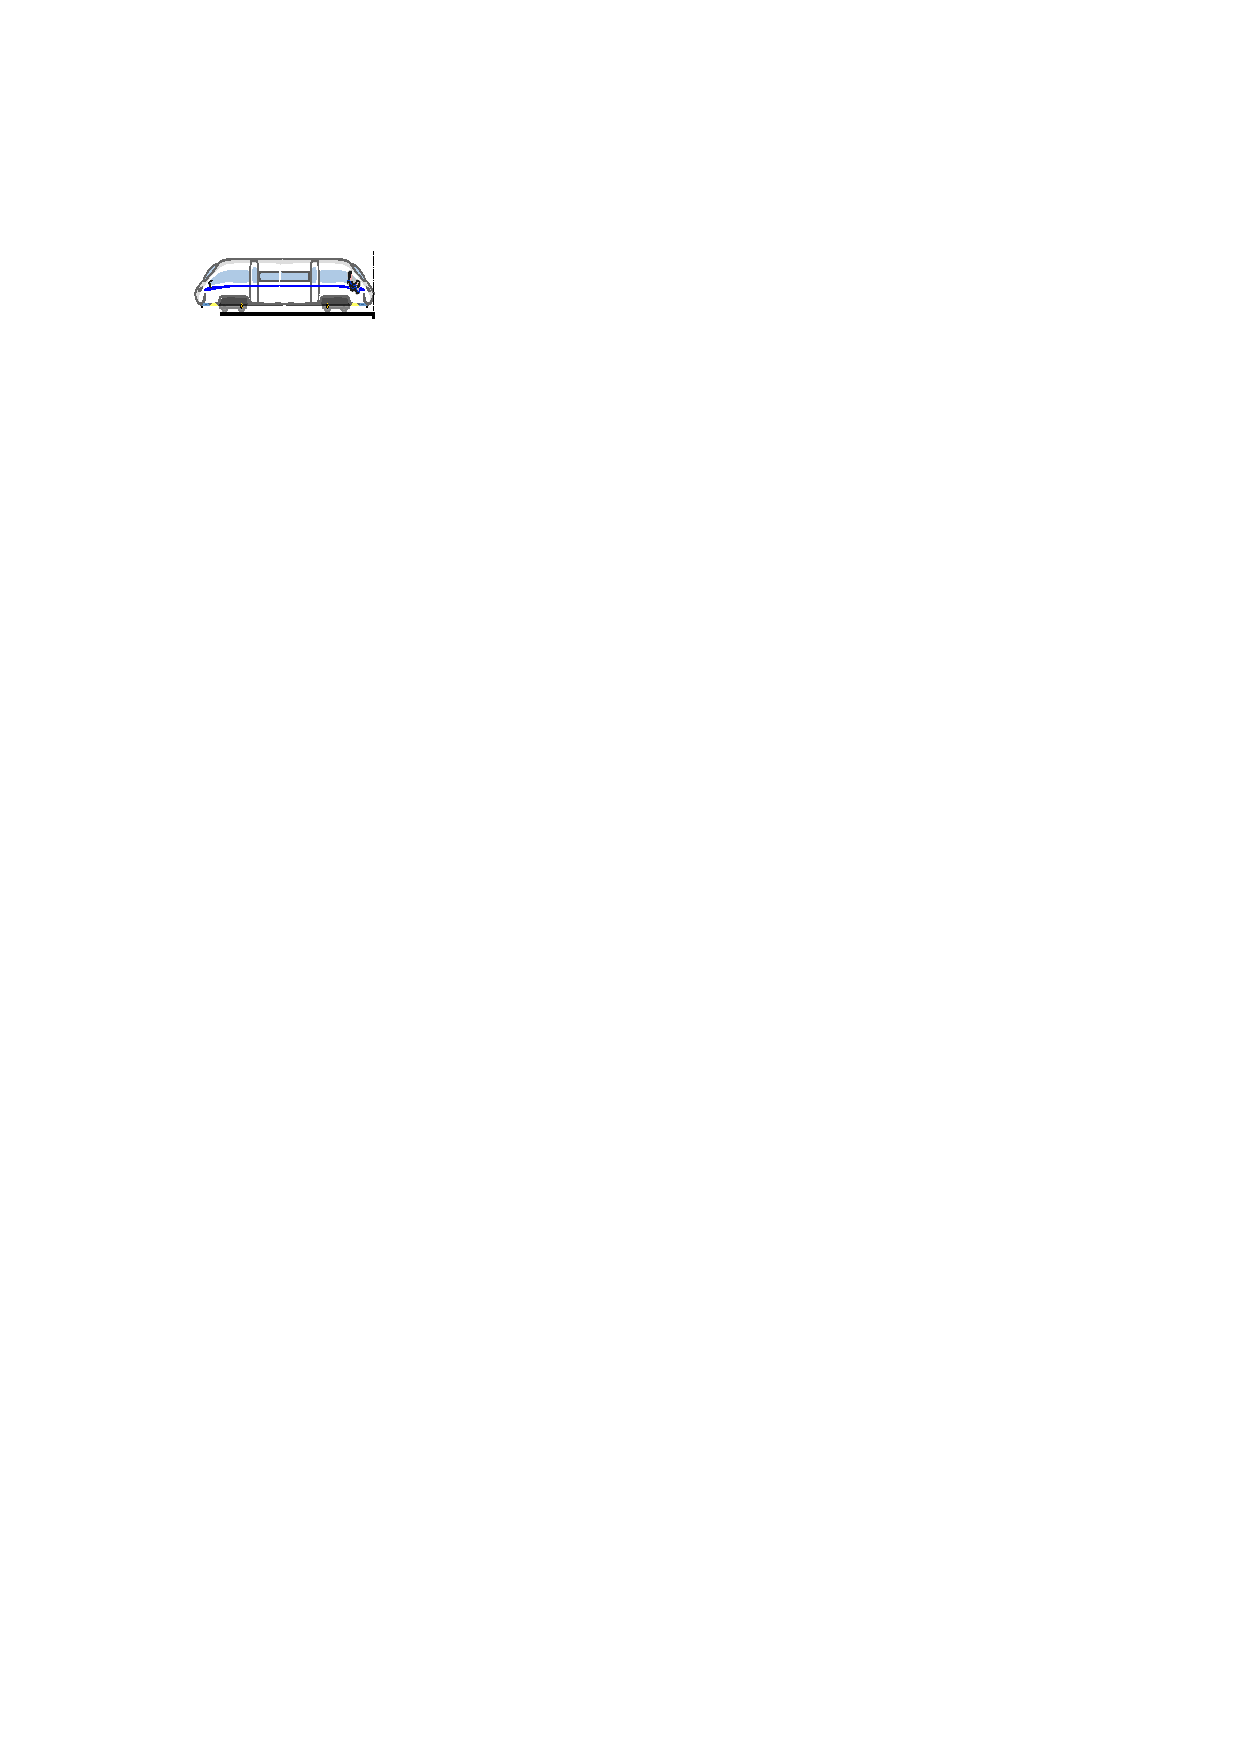
\includegraphics[scale=0.95]{figures/ch2/figure1.pdf}
	\caption{xxx示意图。 \\Fig~\ref{fig:ch2-f1}~Illustration of xxx.}
	\label{fig:ch2-f1}
\end{figure}

\vspace{-2em}

\begin{figure}[!htb]
	\centering
	\setlength{\belowcaptionskip}{-0.2cm} %调整图片caption与正文之间的间距,table用\abovecaptionskip。可自己调整。
	\addtocounter{subfigure}{-1}\subfigure[Subfig1.] {\subfigure[子图1] {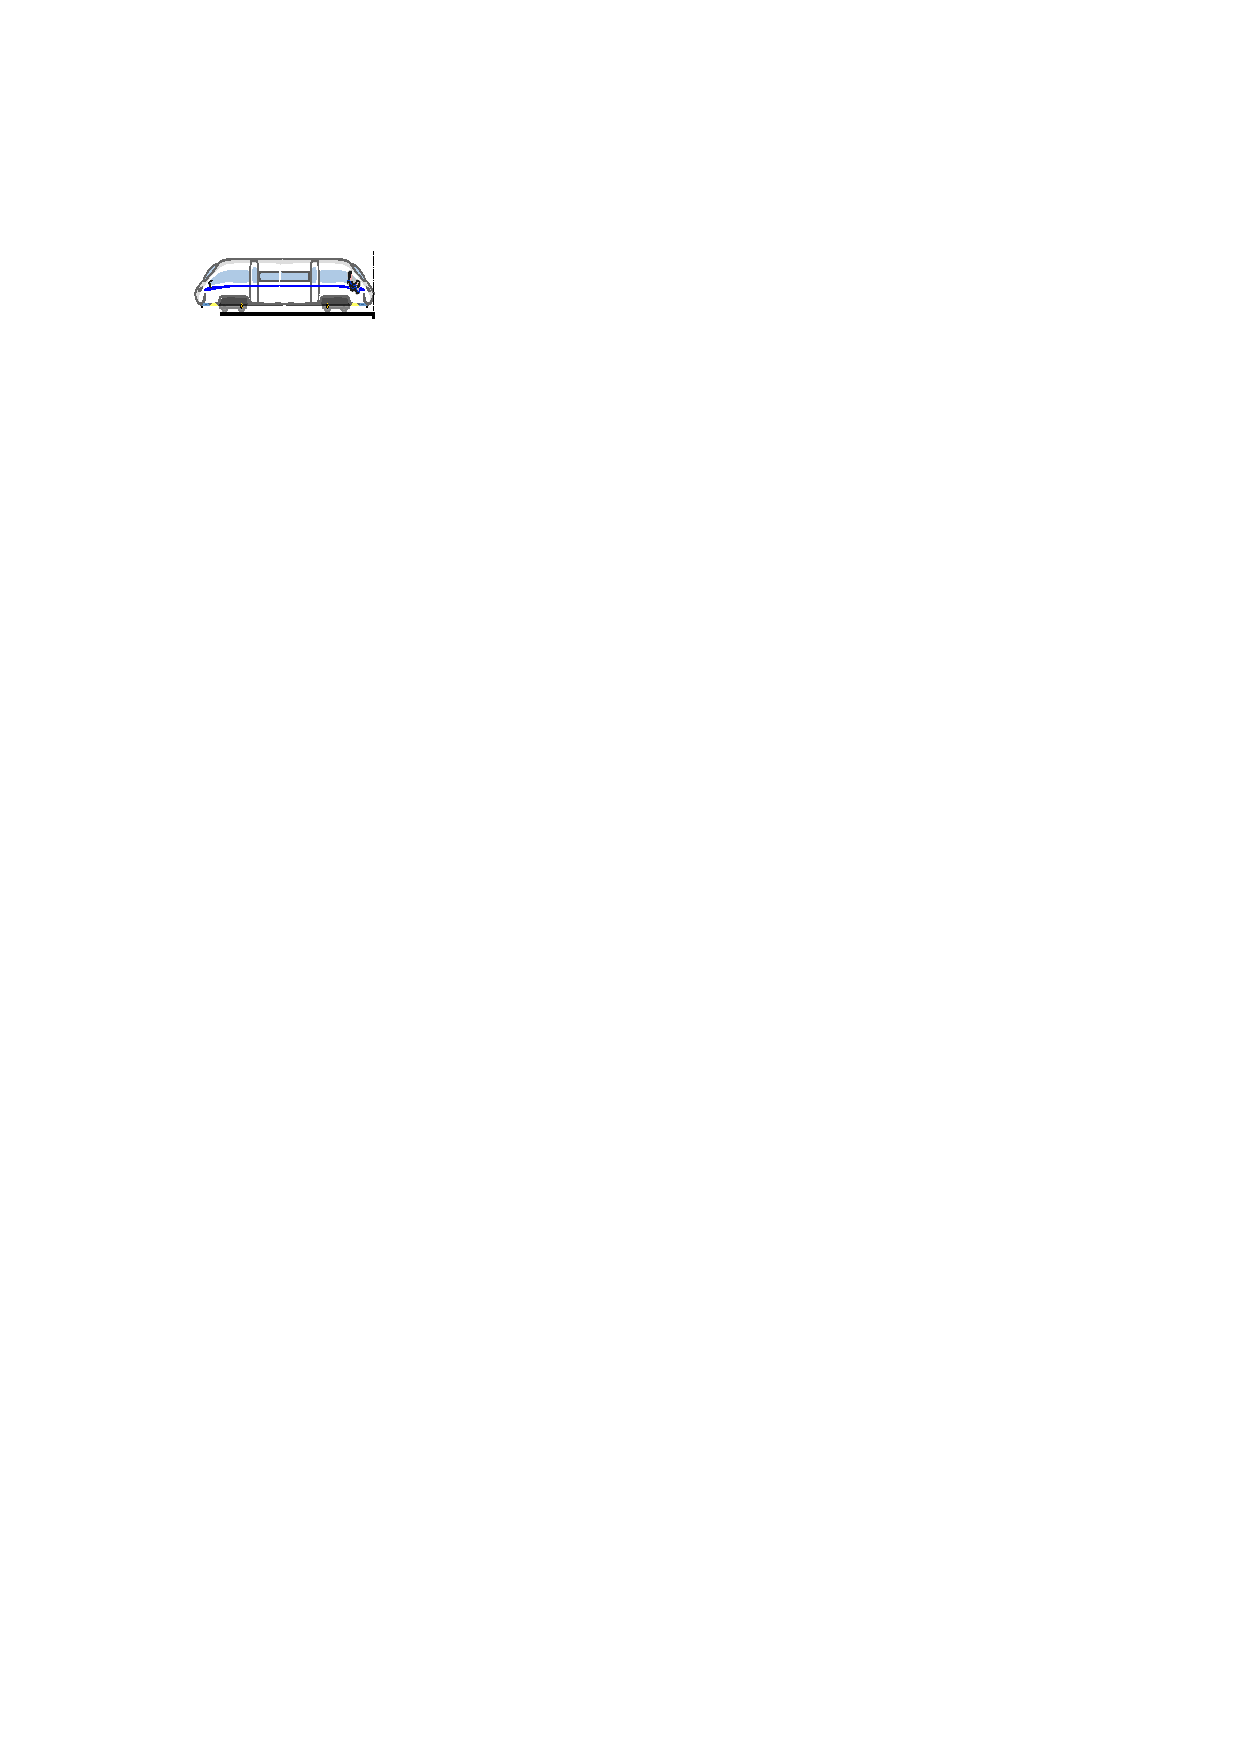
\includegraphics[scale=1]{figures/ch2/figure1.pdf}}}
	\hspace{20pt} %子图间距
	\addtocounter{subfigure}{-1}\subfigure[Subfig2.] {\subfigure[子图2]{ 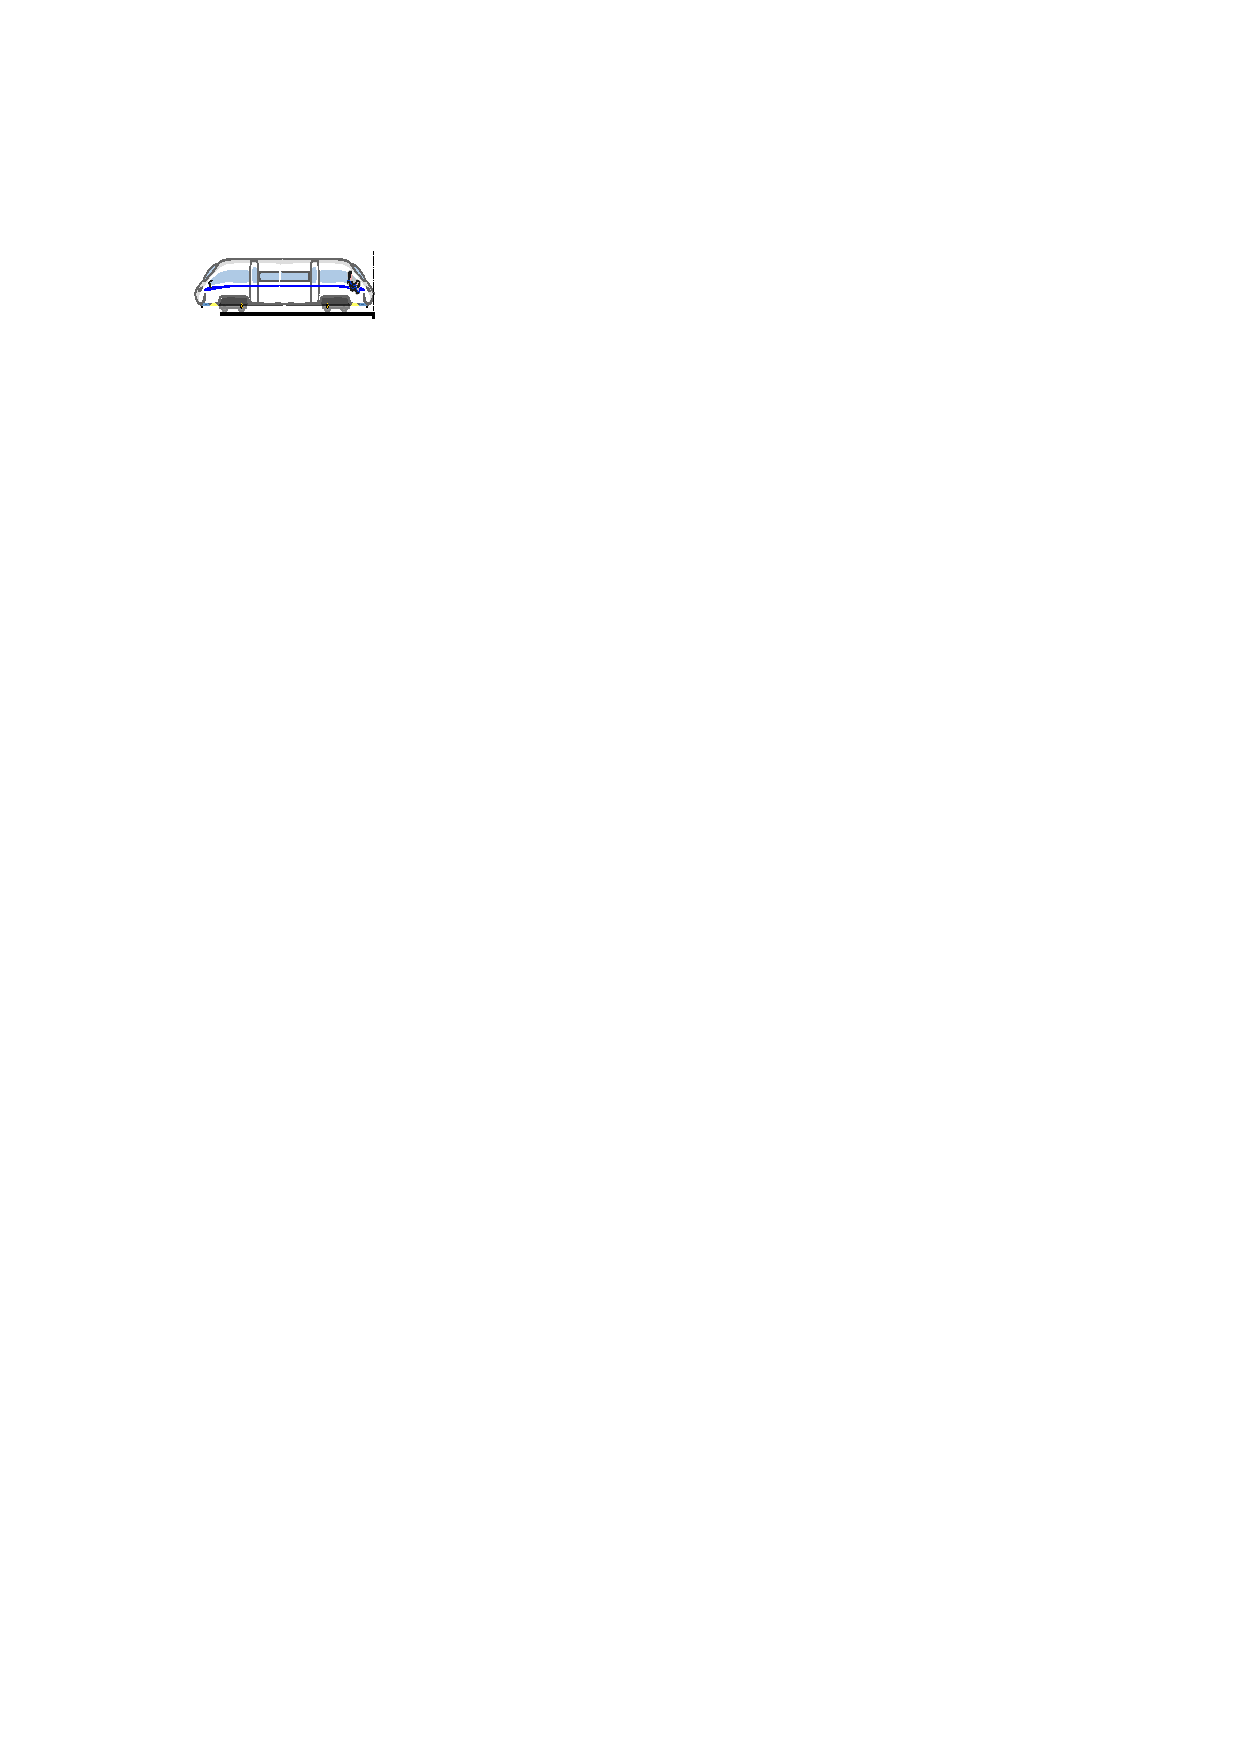
\includegraphics[scale=1]{figures/ch2/figure1.pdf}}}
	\caption{xxx示意图。\\Fig~\ref{fig:ch2-f2}~Illustration of xxx.}
	\label{fig:ch2-f2}
\end{figure} 


